\documentclass{article} 

\usepackage{amsmath}  %调用公式宏包
\usepackage{graphicx} %调用插图宏包
\usepackage{ctex}     %调用中文宏包
\usepackage{ulem}
\usepackage{xcolor}
\setlength{\parindent}{2em}
\usepackage{hyperref}
\usepackage{float}
\hypersetup{hidelinks,
colorlinks=true,
allcolors=blue,
pdfstartview=Fit,
breaklinks=true}
\newCJKfontfamily{\cusong}[AutoFakeBold={2.17}]{SimSun}
\renewcommand{\d}{\mathrm{d}}
%\begin{document}这句话之前是导言区,这句话以后就开始写正文了
%可以把导言区理解为int main()函数之前的内容,而正文就是int main()主函数的部分了
\begin{document}
\begin{titlepage}
    \title{\vspace{-4cm}\textbf{\cusong 中山大学物理与天文学院本科生期末考试}}
    \date{}
    \author{}
\end{titlepage}
\maketitle
\noindent 课程:2023级《物理学前沿》\\
\rightline{所选择的授课教师名字:孙佳睿}
\rightline{(题目):宇宙中的神秘天体:黑洞}
\noindent 学生姓名:姚昊廷 \hfill 学生学号:22322091\\
\noindent 班\ \ \ \ \ \ 别:3班\hfill 联系电话:19171015745\\
%分章节的示例,Latex会自动帮忙给标题编号
\begin{abstract}
    最早在十八世纪,约翰·米歇尔和皮耶-西蒙·拉普拉斯就考虑过引力场强大到光线都无法逃逸的天体。在爱因斯坦提出了他著名的广义相对论场方程$R_{\mu\nu}-\frac{1}{2}Rg_{\mu\nu}=\frac{8\pi G}{c^4}T_{\mu\nu}$后,探求该
    方程的解析解便成了无数物理学家毕生追求的任务。1916年,在一战的战壕中,卡尔·施瓦西首个给出了这个场方程除平直时空以外的解析解。
    然而史瓦西解的给出带来了一个新的奇点,在理论上首次预言了黑洞这种神奇的天体。2016年2月11日,LIGO科学合作组织和Virgo合作组宣布第一次直接观测到引力波,这也代表第一次观测到黑洞合并。
    2019年4月10日,首次发布了黑洞及其附近的第一张影像:使用事件视界望远镜在2017年拍摄到M87星系中心的超大质量黑洞。至此人类终于首次直接观测到宇宙
    中最神秘的天体:黑洞。
    \begin{figure}[H]
        \centering
        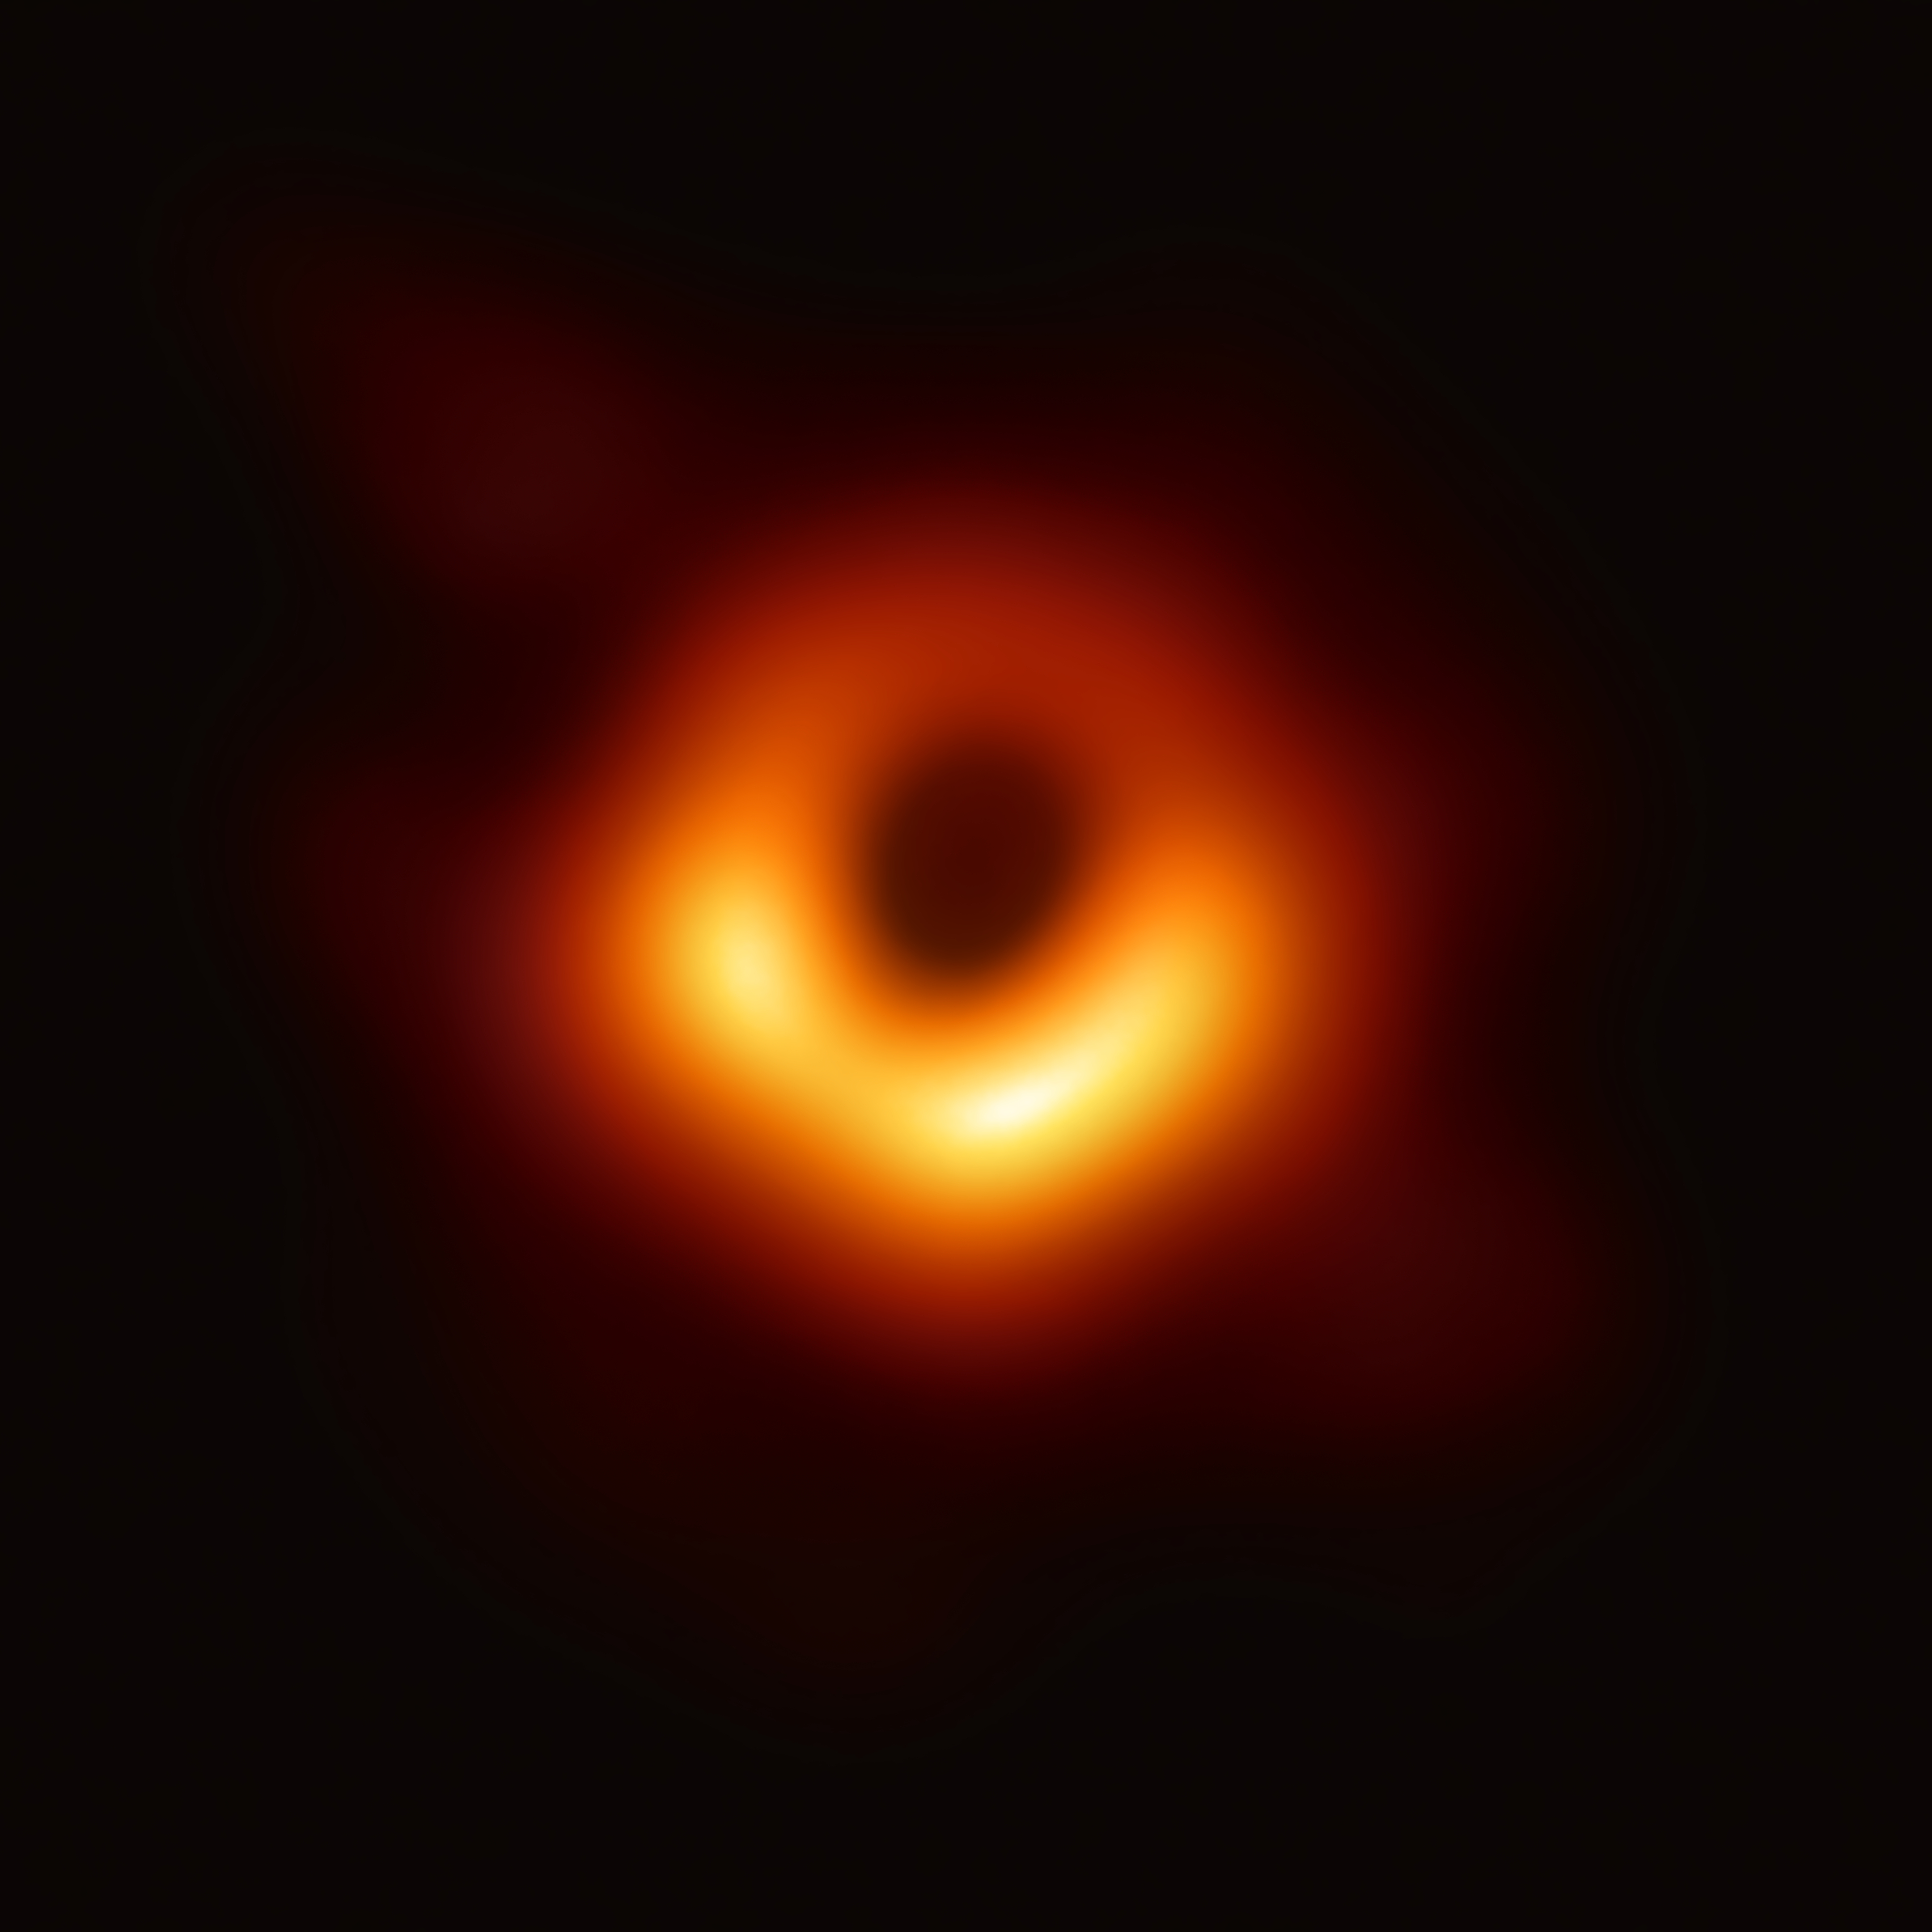
\includegraphics[width=0.5\textwidth]{Black_hole_-_Messier_87_crop_max_res.jpg}
        \caption{人类首张黑洞照片}
    \end{figure}
\end{abstract}
\section{史瓦西解}
在爱因斯坦场方程提出后,因其高度的非线性加之变量耦合,导致求取解析解十分困难。爱因斯坦在给出场方程
的时候只给出了一个最平凡的解:一个无物质的宇宙中的时空处处是平直的。然而此时在一战的战壕中史瓦西给出了其第一个
非平凡解。史瓦西考虑了一个只在宇宙中心有一个质量为$M$的球状物体的宇宙,并且不带电,无自旋。这样的宇宙是球对称的
,史瓦西给出了该宇宙度规的解析解。即
\begin{equation}
    \d s^2=c^2\left(1-\frac{2GM}{c^2r}\right)\d t^2+\frac{\d r^2}{\left(1-\frac{2GM}{c^2r}\right)}+r^2(\d \theta^2+\sin^2\theta\d \phi^2)
\end{equation}
该解在$r\to\infty$或$M\to0$时均退化为闵氏时空,这是合乎物理直觉的。但是这个解表明该宇宙似乎有两个奇点,其中一个处于$r=0$处,这个奇点是容易理解的,因为此处时空曲率无穷大,任何理论在
此处均失效。但是在$r=r_s\equiv\frac{c^2}{2GM}$处,似乎也出现了奇点。在 1924年,亚瑟·爱丁顿构造出了第一个坐标变换,使得史瓦西解在$r=r_s$处没有奇点,
也就是爱丁顿-芬克斯坦坐标(Eddington–Finkelstein coordinates)。后来随着微分几何等一系列数学工具进入物理学研究后
人们才发现$r=r_s$处并不是真正的奇点,正式证明了$r=r_s$处只是时空上的一处事件视界而已。即虽然在黑洞外界人看来穿过事件视界的时间
是无限的,然而对穿过事件视界的人来说,其所经历的固有时是有限的。\par
该解将时空分为了两部分,在$r<r_s$内的物体的未来光锥无法进入$r>r_s$处,也即黑洞内部物体无法影响外部,使用彭罗斯时空
图可以更直观的理解这个结果。
\begin{figure}[H]
    \centering
    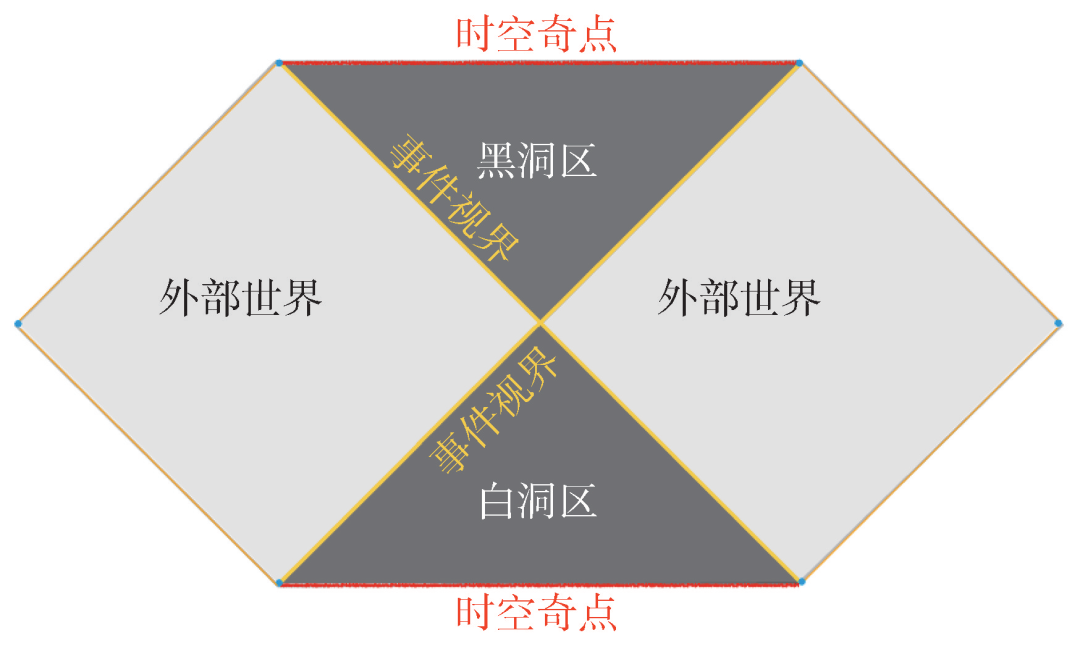
\includegraphics[width=0.5\textwidth]{20210121064530_a51be8.jpg}
    \caption{彭罗斯时空图}
\end{figure}
在彭罗斯时空图中物体的未来光锥为向上的直角区域。从该图可以直观看出物体无法从黑洞逃逸。
\section{黑洞无毛定理}
一旦黑洞在形成后达到稳定状态,黑洞就只有三个独立的物理特性:质量、电荷、和角动量。虽然在广义相对论中黑洞的任何物质都无法脱离,
但是霍金将量子力学与广义相对论结合,指出黑洞也会以热辐射的形式向外辐射。
并且霍金通过计算论证了黑洞只会发出一种辐射,且这种辐射只与质量、电荷、和角动量有关。这个结果就产生了\textbf{\cusong 黑洞信息疑难}
即,如果我们将一段含有这三个参量以外的信息丢入黑洞中,那么其他的信息就会完全失去。然而这违反了我们在经典物理和量子
物理共同的准则即因果律:原则上,一个系统在某个时间点的状态应该决定了其在其他任意时间点的状态。即使在量子物理中
系统的状态也是由其波函数刻画。而波函数的演化由一个幺正算符确定。而幺正性确保了我们可以从任意一个时刻的波函数
确定其之前或之后任意时刻的波函数。但是黑洞的霍金辐射却告诉我们多个不同的系统只要具有相同的质量、电荷、和角动量便
可以演化到同一个状态,而关于初状态的信息完全丢失了,这挑战了因果律。当然,人们还是普遍相信这一部分信息并没有丢失
但是关于这些信息的去向目前仍没有好的解释。近年来,人们研究了该最初悖论的一些扩展版本。这些关于黑洞蒸发的众多难题
牵涉到引力与量子力学该如何结合,使得信息悖论仍然是量子引力中一个活跃的研究领域。
\section{黑洞的探测}
由于黑洞只会发出一种尚未证实的霍金辐射,因此对黑洞的直接观测十分困难。目前人们对黑洞的观测还是主要通过间接
观测来实现。目前最主流的几种观测手段有
\begin{enumerate}
    \item 微引力透镜法:众所周知,强引力可以弯折光的传播路径,因此可以通过引力透镜效应来探寻宇宙中的致密天体,但遗憾的是我们无法有效的分辨出黑洞与其他致密天体。
    \item X射线双星系统
    \item 物质吸积
\end{enumerate}
此外,爱因斯坦预言大质量黑洞的合并过程会对周围时空产生大幅度扰动,产生引力波,引力波是以光速传播的横波。2016年2月11日,LIGO科学合作组织和Virgo合作组宣布第一次直接观测到引力波,这也代表第一次观测到黑洞合并。
这代表人类第一次证明了黑洞的存在。
\section{黑洞的热力学}
1972年,霍金与两位合作者写了一篇关于黑洞力学的论文,他们在论文中指出,一个黑洞的力学性质可以只用两个参数
来表征:黑洞的面积(即视界的面积,对于史瓦西黑洞而言$A=4\pi r_s^2$)和视界的表面引力(单位质量物体在视界表面
获得的引力加速度表征即$g=GM/r_s^2$)。这两个参量类似于热力学中的熵和温度,基于这种相似性,他们仿照热力学四定律提出了
黑洞的力学四定律。表述为
\begin{enumerate}
    \item 第零定律:平衡状态的黑洞视界上所有的点具有相同的表面引力;
    \item 第一定律:黑洞演化过程中,质量、转动速度和角动量的演化都可以写为视界面积和表面引力的函数;
    \item 第二定律:宇宙中所有黑洞面积之总和不会随时间减小;
    \item 第三定律:经过有限次转换把黑洞表面引力降低为0是不可能的。
\end{enumerate}
第二定律让我们想起热力学中的熵增定律。贝肯斯坦在1973年证明,黑洞质量$M$的变化与视界面积$A$的变化存在关系
\begin{equation}
    \d M=T\d \left(\frac{kc}{4\pi\bar{h}G}A\right)
    \label{1}
\end{equation}
其中$\bar{h}$是普朗克常数,$k$是玻尔兹曼常数。这个关系使我们想起热力学第一定律
\begin{equation}
    \d E=T\d S
    \label{2}
\end{equation}
又因为$E=Mc^2$,因而\ref{1}中的$T$应为热力学温度,$A$就应与热力学熵$S$成正比,即
\begin{equation}
    S=\frac{kc^3}{4\pi\bar{h}G}A
\end{equation}
在史瓦西黑洞的情况下
\begin{equation}
    A=4\pi r_s^2=\frac{16\pi G^2M^2}{c^4}
\end{equation}
因为$S\propto A$,故
\begin{equation}
    \delta S\propto \delta A\Rightarrow \delta S\propto M\delta M
    \label{3}
\end{equation}
取$c=1$单位制,则$E=M$,则由\ref{2}和\ref{3}知道
\begin{equation}
    \delta M=T\delta S\propto TM\delta M
\end{equation}
这个式子表明
\begin{equation}
    TM=const\Rightarrow T\propto \frac{1}{M}
\end{equation}
可见质量越小的黑洞温度越高。
%参考文献部分
\begin{thebibliography}{最宽序号}
    \bibitem[1]{检索名 1}向守平.天体物理概论[M].合肥:中国科学技术大学出版社,2008.11(2022.11重印)
    \bibitem[2]{检索名 2}孙佳睿.frontier course-fantastic black hole.珠海
    \bibitem[3]{检索名 2}J-P·卢米涅.黑洞.卢炬甫译.长沙:湖南科学技术出版社,1997
\end{thebibliography}

\end{document}